\documentclass[11pt,a4paper,twoside,notitlepage]{article}
%comment out the line above and decomment the one below; the format will change
%\documentclass[conference,a4paper]{IEEEtran}  

%
% Here, you specify the packages you need
%

%You need these 2 packages to write algorithms
\usepackage{algorithmic}
\usepackage{algorithm}
%You need this package to handle figures
\usepackage{graphicx}
%You need this package to write Romanian diacritics properly
\usepackage{combelow}
\usepackage{hyperref}

\usepackage[utf8x]{inputenc} %alternative solution for Romanian diacritics
%This is how you define you own commands/macros
%this is a macro for writing "n choose k" the Romanian style
\newcommand{\mycomb}[2]{{C}_{#1}^{#2}} 
%this is a macro for writing "n choose k" the English style
%\newcommand{\mycomb}[2]{\left( \begin{array}{l}{#2}\\{#1}\\ \end{array} \right)} %this 


%
% The document content starts here
%
\setcounter{tocdepth}{2}
\renewcommand{\contentsname}{Cuprins}
%\setlength{\parindent}{4em}

\begin{document}
% paper title 
\title{Bontida are nevoie de ajutor}

% author names and affiliations
\author{
Student: Gabor George C\u{a}t\u{a}lin\\ %double backslash means linebreak
Grupa: 30239\\
}

%generate paper title
\maketitle 

\newpage

\tableofcontents

%\section*{Cuprins}


\newpage

\section{Analiza cerințelor}

\subsection{Specificare cerinte}
Se cere realizarea unei aplicatii desktop pentru vanzarea de bilete pentru festivalul Electric Castle. Aceasta va avea doua tipuri de utilizatori: 
\begin{itemize}
	\item administrator;
	\item casier.
\end{itemize}
si patru tipuri de bilete:
\begin{itemize}
	\item Ziua 1, pret 200 RON;
	\item Ziua 2, pret 200 RON;
	\item Ziua 3, pret 200 RON;
	\item Toate zilele, pret 400 RON.
\end{itemize}
De asemenea, in fiecare zi pot fi un numar maxim de oameni la festival.


\subsection{Cerinte functionale}
Aplicatia trebuie sa puna la dispozitie utilizatorilor urmatoarele functionalitati:
\begin{itemize}
	\item autentificarea prin LOGIN si redirectionarea la operatii specifice utilizatorului;
	\item pentru casier:
					\begin{itemize}
						\item	vanzarea de bilete si crearea automata a unui fisier pe disk cu detalile biletului. In momentul cand este vandut un bilet urmatoarea constrangere trebuie respectate: Biletele din Ziua x + Biletele Toate zilele \textless  MAX\_CAPACITY;
						\item 	Vizionarea istoricului biletelor vandute de catre el ordonate dupa timp+data (ultimele bilete vandute fiind primele).
					\end{itemize}
	\item pentru administrator:
					\begin{itemize}
						\item	operatii CRUD pe casier;
						\item	Modificarea numarului MAX\_CAPACITY;
						\item	Raport cu numarul de bilete vandute per casier;
						\item	Raport cu incasarile pe zi + totale bazate pe biletele vandute.
					\end{itemize}
\end{itemize}

\subsection{Cerinte non-functionale}
Urmatoarele cerinte trebuie respectate:
\begin{itemize}
	\item	timpul de raspuns al sistemului pentru orice operatie trebuie sa fine mai mic de 2 secunde;
	\item	arhitectura sistemului trebuie sa permina adaugarea de noi operatii sau modificarea celor curente;
	\item	sistemul trebuie sa fie interactic, sa ofere mesaje utilizatorului pentru al ghida.
\end{itemize}


\section{Use Case Model}

Use case: Vanzare bilet; \\
Level: User-goal; \\
Actor princital: Casier; \\
Scenariu de succes: casierul se logheaza, alege tipul biletului si apasa butonul pentru vanzare. Un mesaj este afisat pentru a confirma reusita operatiei; \\
Extensii: Operatia nu poate esua decat daca intervine o problema in baza de date. \\
\newpage
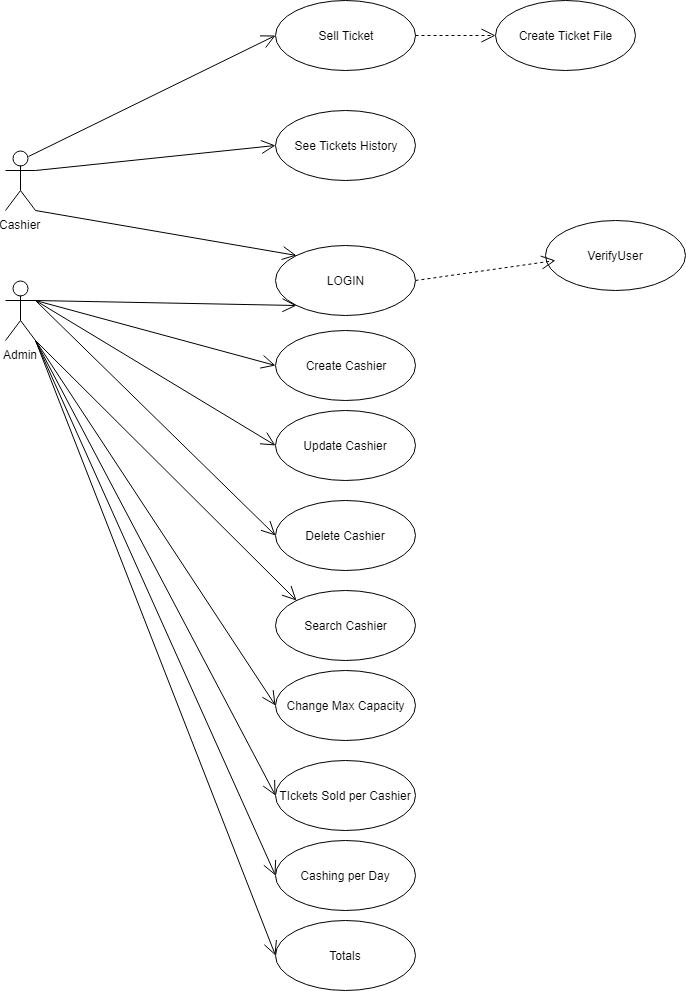
\includegraphics[height=.5\textheight]{UseCases}


\section{Design-ul arhitectural al sistemului}

\subsection{Descrierea modelului arhitectural}
Este utilizat pattern-ul arhitectural Layers.\\
Aplicatia este compusa din trei nivele: 
\begin{itemize}
	\item Presentation - contine interfata cu utilizatorul; 
	\item Logic - structurile de date necesare pentru realizarea operatilor;
	\item DataAccess - conexiunea cu baza de date si extragerea, schimbarea datelor din aceasta.
\end{itemize}

\subsection{Diagrame}

Urmatoarea diagrama prezinta structura pachetelor din sistem :
\newpage
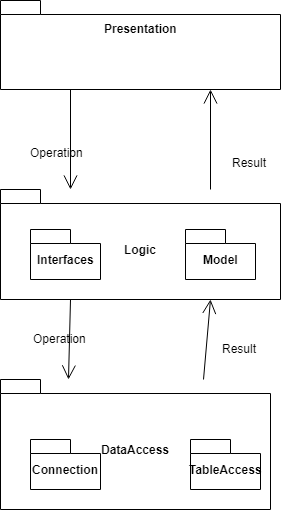
\includegraphics[height=.4\textheight]{Packages} \\ 
Diagrama de componente: \\
\\
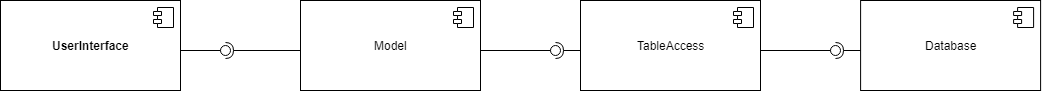
\includegraphics[width=.6\textheight]{Component} \\
Diagrama de deployment: \\
\\
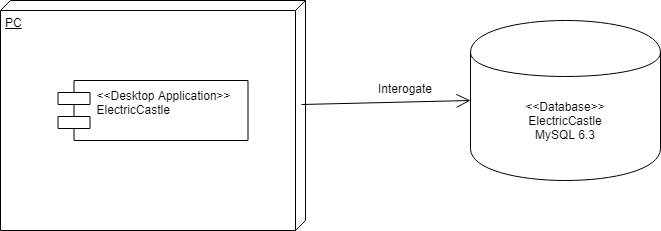
\includegraphics[width=.6\textheight]{Deployment} \\


\section{Diagrame de secventa UML}
Consideram scenariul in care un anumit casier doreste sa vada lista cu biletele vandute de el. Avem urmatoarea diagrama de secventa: \\
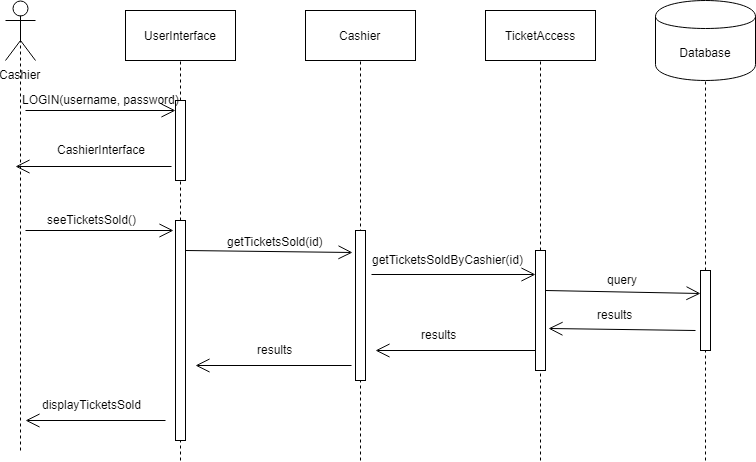
\includegraphics[width=.6\textheight]{Sequential}


\section{Design-ul claselor}

\subsection{Descriere design pattern-uri utilizate}

Au fost utilizate urmatoarele:
\begin{itemize}
	\item Data Mapper - Clasele User, Ticket, Cashier si Admin nu contin interogari SQL sau connexiuni la baza de date. Toate datele care trebuie scrise sau citite sunt transferate prin clasele TicketAccess si UserAccess;
	\item Singleton - Exista o singura instanta a clasei ConnectionFactory;
	\item Delegation - Clasele acceseaza metode doar ale claselor vecine.
\end{itemize}

\newpage
\subsection{Diagrama de clase}
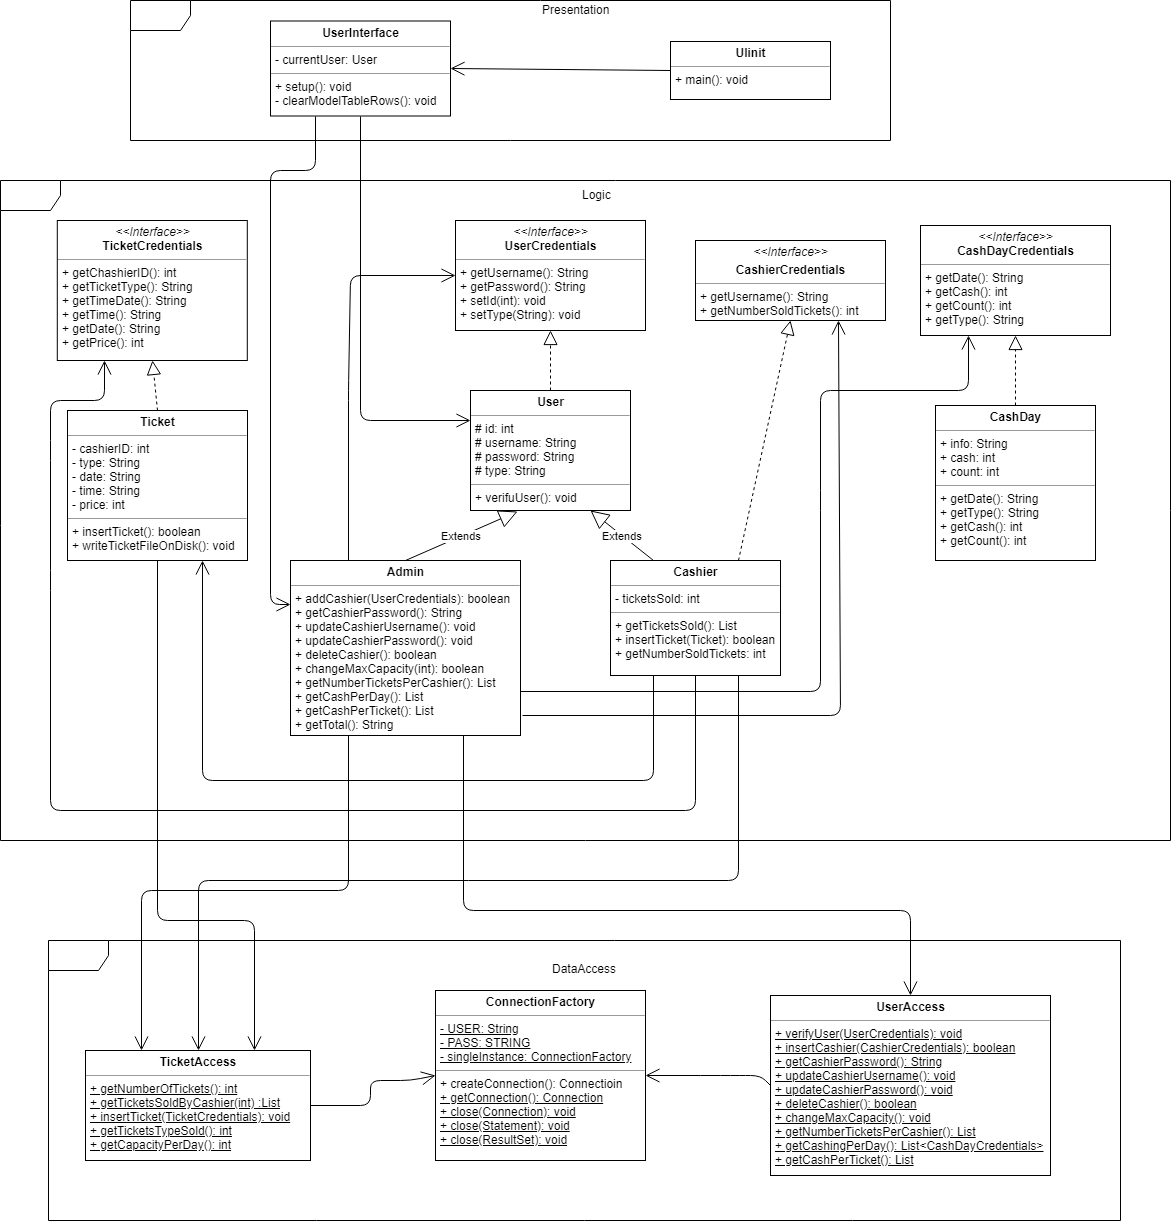
\includegraphics[height=.75\textheight]{ClassDiagram}

\section{Model de date}

Baza de date in care sunt stocate informatiile este urmatoare: \\
\includegraphics[height=.3\textheight, width=.8\textwidth]{Database} \\
Dupa cum se poate, vedea exista patru tabele:
\begin{itemize}
	\item User - atributul "type" este folosit pentru a diferentia intre casieri si administrator;
	\item Ticket - modeleaza tipurile de bilete, atributul "type" reprezinta perioada de access la festival, exemplu "Day1";
	\item Ticketdetails - folosit pentru a evita relatia de n la n intre tabelele User si Ticket si asociaza casierul cu tipul biletului vandut;
	\item Constants - are un singur rand si un singur atribut pentru a retine capacitatea maxima de persoana pentru festival.
\end{itemize}


\section{Testarea sistemului}

S-a folosit o strategie de testare incrementala, functionalitatile au fost verificate pe masura ce au fost adaugate in sistem. Astfel, principalele metode de testare au fost data-flow (au fost date anumite intrari si s-a observat raspunsul sistemului), white-box (codul a fost disponibil) si boundary analysis (pentru valoarea capacitatii intr-o zi de festival).

\section{Bibliografie}

Pentru UML:
\begin{itemize}
	\item \url{https://www.youtube.com/watch?v=OkC7HKtiZC0&list=PLGLfVvz_LVvQ5G-LdJ8RLqe-ndo7QITYc}  \\
\end{itemize}
Pentru anumite erori, pattern-uri:
\begin{itemize}
	\item \url{https://stackoverflow.com/}
	\item \url{https://www.youtube.com/}	
	\item \url{https://en.wikipedia.org/wiki/Main_Page}
\end{itemize}

\end{document}
